\documentclass{beamer}


\usepackage{color}
\usepackage{listings}
\usepackage{courier}
\lstset{
basicstyle=\tiny\ttfamily, % Standardschrift
numbers=left, % Ort der Zeilennummern
tabsize=4, % Groesse von Tabs
}
\lstloadlanguages{C++}
%\DeclareCaptionFont{blue}{\color{blue}}
 
%\captionsetup[lstlisting]{singlelinecheck=false, labelfont={blue}, textfont={blue}}
\usepackage{caption}
\DeclareCaptionFont{white}{\color{white}}
\DeclareCaptionFormat{listing}{\colorbox{8}{\parbox{\textwidth}{\hspace{15pt}#1#2#3}}}
\captionsetup[lstlisting]{format=listing,labelfont=white,textfont=white, singlelinecheck=false, margin=10pt, font={bf,footnotesize}}

\usepackage[utf8x]{inputenc}
\usepackage{ngerman}
\usepackage{graphicx}
\usepackage{amsmath}
\usepackage{amssymb}




\title{Diskrete Minimalflächen}
\author{Matthias Hofmann, Michael Rehme und Nadine Schlotz}
\date{\today}

\usepackage{beamerthemesplit}


\begin{document}

\begin{frame}
	\titlepage
\end{frame}

\section{Allgemeines}

\begin{frame}
	\frametitle{Die Aufgabenstellung}
	\begin{figure}
	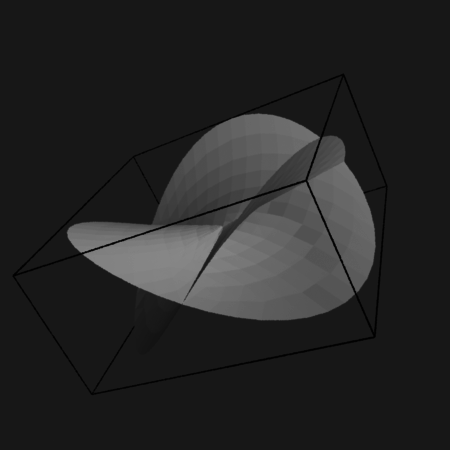
\includegraphics[scale=0.2]{Schneiden.png} \hspace{1cm}
	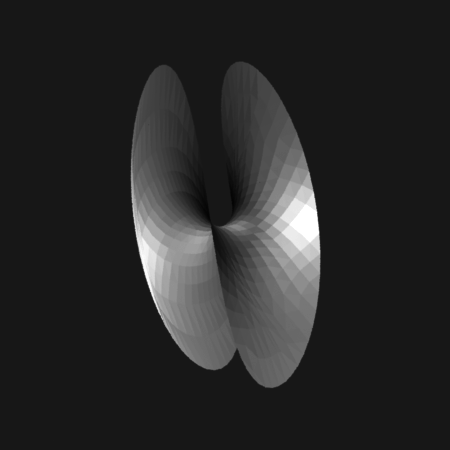
\includegraphics[scale=0.2]{Tennisballkurve.png}
	\end{figure}
	\begin{quote}
		„Beschreiben Sie eine triangulierte Fläche in eine gegeben gekrümmte Raumkurve ein und versuchen Sie, eine Approximation an eine Minimalfläche zu berechnen.“
	\end{quote}
\end{frame}

\begin{frame}
\frametitle{Vorgehensweise}
\begin{itemize}
\item Einbeschreibung einer Fläche $\Longrightarrow$ Triangulierung.
\item Einzelschrittverfahren zur Minimierung des Gesamtoberflächeninhalts
\item Darstellung mittels \texttt{Geomview}
\end{itemize}
Hierfür benötigen wir noch eine geeignete Struktur.
\end{frame}
\section{Strukturelemente}
\subsection{klassen.h}

\begin{frame}[fragile]
\frametitle{klassen.h}

\begin{lstlisting}
#ifndef KLASSEN_H_
#define KLASSEN_H_

#include <iostream>
#include <fstream>
#include <list>
#include<vector>
#include<cstdlib>
#include<math.h>

using namespace std;

const unsigned int dim=3;

class Gitter; //forward declaration
\end{lstlisting}

\end{frame}

\begin{frame}[fragile]
\begin{lstlisting}
//Vektor
class victor {
    public:
		bool isRand;
        vector<double> v;
        list<pair<int, int> > dreiecke;
        victor();
        victor(const vector<double> arg);

        victor& operator+=(const victor& arg);
        victor operator+(const victor& arg)const;

        victor operator-(const victor& arg)const;
        victor& operator-=(const victor& arg);

        victor& operator*=(const double& arg);
        victor operator*(const double& arg)const;

        victor& operator/=(const double& arg);
        victor operator/(const double& arg)const;


        double operator*(const victor& arg)const;

        void clear();

        void ausgeben();
};
\end{lstlisting}
\end{frame}

\begin{frame}[fragile]
\begin{lstlisting}
//Dreieck
class Dreieck
{
    public:
		Dreieck();
        Dreieck(Gitter* vater);
        Dreieck(Gitter* vater,int a, int b, int c);
        virtual ~Dreieck();
        int punkte[3];
        Gitter* papa;
\begin{lstlisting}
//Dreieck
class Dreieck
{
    public:
		Dreieck();
        Dreieck(Gitter* vater);
        Dreieck(Gitter* vater,int a, int b, int c);
        virtual ~Dreieck();
        int punkte[3];
        Gitter* papa;
\end{lstlisting}
\end{frame}

\begin{frame}[fragile]
\begin{lstlisting}
//Dreieck
class Dreieck
{
    public:
		Dreieck();
        Dreieck(Gitter* vater);
        Dreieck(Gitter* vater,int a, int b, int c);
        virtual ~Dreieck();
        int punkte[3];
        Gitter* papa;

        // gibt die flaeche des dreiecks zurueck
        double flaeche();
        // gibt den gradienten an einer ecke (also 0 = 1. ecke, 1 = 2. ecke,
        // 2 = 3. ecke) zurueck
        victor gradient(int ecke);
};
\end{lstlisting}
\end{frame}

\begin{frame}[fragile]
\begin{lstlisting}
//Punkteklasse
class Punkt
{
    public:
        Punkt();
        Punkt(victor v, double t);
        virtual ~Punkt();
        Punkt& operator=(const Punkt& other);

        victor Ort;
        double parameter;
};
\end{lstlisting}
\end{frame}

\begin{frame}[fragile]
\begin{lstlisting}
//Gitter
class Gitter
{
    public:
        Gitter();
        Gitter(const vector<Punkt> arg1,const vector<Dreieck> arg2 );
        Gitter(int mode);
        std::vector<Punkt> gib();
        virtual ~Gitter();
        std::vector<Punkt> punkte;
        std::vector<Dreieck> dreiecke;

        void finde();
        victor gradient(Dreieck* arg, int ecke);
        double Oberflaeche();
        void verbessere();
        void verbessere(int arg);
        void Verfeinere(int mode);
        void Verfeinere(int mode, int arg);
};
\end{lstlisting}
\end{frame}

\begin{frame}[fragile]
\begin{lstlisting}
//Methods
double norm(const victor& arg);
void vcout(victor arg);
void Gcout(const Gitter& arg);
victor def(double a, double b);
victor def(double a, double b,double c);
victor cross(victor a, victor b);
victor randkurve(double t, int mode);
Punkt randpunkt();
\end{lstlisting}
\end{frame}

\begin{frame}
\frametitle{Zusammenfassung}
\begin{itemize}
\item Wir haben eine Vektorenklasse \texttt{victor} und verfügen über Grundrechenarten, Skalarprodukt und Kreuzprodukt. 
\item Die Punkteklasse \texttt{Punkt} basiert im wesentlich aus einem Vektor und einem Paramter zur zugehörigen Parametrisierung.
\item Wir unterscheiden zwischen Rand- und inneren Punkten. Randpunkte bleiben fest und sind durch den Wahrheitswert isRand zu erkennen.
\end{itemize}
\end{frame}

\begin{frame}
\begin{itemize}
\item Unter Dreiecken verstehen wir ein Trippel aus Indizes der Punkteliste. 
\item Im Gitter sammeln wir eine Punkte- und Dreiecksliste. Insbesondere kann \texttt{Gitter::Oberflaeche()} die  Oberfläche der Triangulierung berechnen.
\item Zudem besitzt jeder Punkt über den Vektor \texttt{Ort} eine Liste sämtlicher anliegender Dreiecke. Die Erstellung dieser Liste erfolgt durch \texttt{Gitter::finde()}.
\item Die Triangulierung wird in \texttt{Gitter::Verfeinere()} bewerkstelligt.
\item Das Einzelschrittverfahren zur Minimierung wird in \texttt{Gitter::verbessere()} implementiert.
\end{itemize}
\end{frame}
\section{Die Methoden}
\subsection{Verfeinerung}
\begin{frame}[fragile]
\frametitle{Triangulierung}
Für gegebene Parametrisierung $\gamma: [0,1]\rightarrow \mathbb{R}^3$ einer geschlossenen Kurve erhält man eine Starttriangulatur, als das Dreieck gegeben durch $\gamma(\frac{1}{3}), \gamma(\frac 2 3), \gamma(1)$.
\end{frame}

\begin{frame}
\frametitle{Verfeinerung}
\begin{enumerate}
\item Halbiere jede Seite
\item Verschiebe ihn gegebenfalls auf den Rand ($p_{\text{neu}} =\frac{p_1+p_2}{2}$), falls es sich um eine Randkante handelt. (Trick: Betrachte Anzahl umliegender Dreiecke)
\item Erzeuge neue Dreiecke aus den eben definierten Punkten.
\end{enumerate}
\end{frame}

\subsection{Gitter::Verfeinere()}
\begin{frame}[fragile]
\frametitle{Gitter::Verfeinere()}

\begin{lstlisting}
//Sucht zu allen Punkten die zugehoerigen Dreiecke
void Gitter::finde() {
    // leere Listen
    for (unsigned int j = 0; j < punkte.size(); j++) {
        punkte[j].Ort.dreiecke.clear();
    }
    for (unsigned int i = 0; i < dreiecke.size(); i++) {
        punkte[dreiecke[i].punkte[0]].Ort.dreiecke.push_back(make_pair(i, 0));
        punkte[dreiecke[i].punkte[1]].Ort.dreiecke.push_back(make_pair(i, 1));
        punkte[dreiecke[i].punkte[2]].Ort.dreiecke.push_back(make_pair(i, 2));
    }
}
\end{lstlisting}
\end{frame}

\begin{frame}[fragile]
\begin{lstlisting}
//Verfeinerungsalgorithmus in Kooperation mit den anderen Grupppen, leicht modifiziert
void Gitter::Verfeinere(int mode) {
 // enthaelt zu (a,b) den Punkt c.Ort = (a.Ort+b.Ort)/2, wobei a,b,c 
 //mithilfe von punktindizes definiert werden
std::map<std::pair<int, int>, int> erstelltepunkte;
std::vector<Dreieck> neuedreiecke = std::vector<Dreieck>();
int pcnt = 0;
int dcnt = 0;
for (unsigned int i = 0; i < dreiecke.size(); ++i) {
int np[3];
for (int j = 0; j < 3; ++j) {
    int a = dreiecke[i].punkte[j];
    int b = dreiecke[i].punkte[(j + 1) % 3];

    if (erstelltepunkte.find(std::pair<int, int>(a, b)) == erstelltepunkte.end()
               && erstelltepunkte.find(std::pair<int, int>(b, a))
                      == erstelltepunkte.end()) {
        Punkt c = Punkt();
        c.Ort = (punkte[a].Ort + punkte[b].Ort) * 0.5;
        if (punkte[a].parameter < punkte[b].parameter)
            c.parameter = (punkte[a].parameter + punkte[b].parameter) * 0.5;
        else
            c.parameter = (1.0 + punkte[a].parameter + punkte[b].parameter)*0.5;
\end{lstlisting}
\end{frame}

\begin{frame}[fragile]
\begin{lstlisting}
        np[j] = punkte.size();
        c.Ort.isRand = 0;
        punkte.push_back(c);
        pcnt++;
        erstelltepunkte.insert(
        std::pair<std::pair<int, int>, int>(std::pair<int, int>(a, b),np[j]));
        } else {
        if (erstelltepunkte.find(std::pair<int, int>(a, b))
            == erstelltepunkte.end()) {
            np[j] = erstelltepunkte[std::pair<int, int>(b, a)];
            } else {
                 np[j] = erstelltepunkte[std::pair<int, int>(a, b)];
        }
    }
}
\end{lstlisting}
\end{frame}

\begin{frame}[fragile]
\begin{lstlisting}
// neue dreiecke erstellen
for (int k = 0; k < 3; ++k) {
    Dreieck d = Dreieck(this, dreiecke[i].punkte[k], np[k], np[(k + 2) % 3]);
    neuedreiecke.push_back(d);
    dcnt++;
}
Dreieck e = Dreieck(this, np[0], np[1], np[2]);
neuedreiecke.push_back(e);
dcnt++;
}
dreiecke = neuedreiecke;
std::cout << "Erstellte " << pcnt << " neue Punkte und " << dcnt
    << " neue Dreiecke" << std::endl;

this->finde();
 //Wenn ein Punkt in weniger als 6 Dreiecken vertreten ist, ist es ein Randpunkt
for (unsigned int i = 0; i < punkte.size(); i++) {
if (punkte[i].Ort.dreiecke.size() < 6) {
    punkte[i].Ort = randpunkt(punkte[i].parameter, mode).Ort;
    punkte[i].Ort.isRand=1;
}
}
}
\end{lstlisting}
\end{frame}
\subsection{Minimierung}

\begin{frame}
\frametitle{Gradientenverfahren}
\begin{itemize}
\item Zu einer gegebenen Triangulierung, soll an dieser Stelle das Gitter optimiert werden. $\Longrightarrow$ Minimierung des Flächeninhalts aller angrenzenden Dreiecke eines Punktes.
\item Für diese Optimierungsaufgabe lässt sich ein Abstiegsverfahren/Näherungsverfahren ausnutzen.
\end{itemize}  
\end{frame}

\begin{frame}
\frametitle{Flächeninhalt eines Dreiecks}
Der Flächeninhalt eines Dreiecks $a, b, c$ berechnet sich zu:
\[
	A=\frac 1 2 |(b-a)\times(c-a)|
\]
Der Gradient zeigt in Richtung Höhe des Dreiecks. (ohne Beweis) Also:
\[
	\nabla_a A\varpropto ((c-a) \times (c-b)) \times (c-b)
\]
Die Gesamtgradientenrichtung ergibt sich dann durch Aufsummation. Für das Abstiegsverfahren negieren wir.
\end{frame}
\subsection{Gitter::verbessere()}
\begin{frame}[fragile]
\frametitle{Gitter::verbessere()}
\begin{lstlisting}
//Berechnet den Gradienten an einem gegebenen Eck.
victor Dreieck::gradient(int ecke)
{
    victor a = papa->punkte[punkte[(ecke+1)%3]].Ort-papa->punkte[punkte[ecke]].Ort;
    victor b = papa->punkte[punkte[(ecke+1)%3]].Ort-papa->punkte[punkte[(ecke+2)%3]].Ort;

    victor c = cross(cross(a,b),b);
    double nc = norm(c);
    if(nc <= 0.0001)return def(0,0,0);
    return c*(norm(b)/norm(c));
}

//Berechnet die Oberflaeche der Gitterstruktur
double Gitter::Oberflaeche() {
	double neuegesamtflaeche=0;
	for(int i = 0; i < dreiecke.size(); ++i)
	        {
	            neuegesamtflaeche += dreiecke[i].flaeche();
	        }
	return neuegesamtflaeche;
}
\end{lstlisting}
\end{frame}

\begin{frame}[fragile]
\begin{lstlisting}
// Verbessert das Gitter
void Gitter::verbessere() {
	victor grad, grad_tmp, tmp;
	double flaeche_ref;
	double flaeche;
	double faktor; //Schrittweite
	double armijo=0.01; //Armijo-koeffizient
	double neueflaeche=this->Oberflaeche();
	double alteflaeche;
	do {
		alteflaeche=neueflaeche;
	for (unsigned int i = 0; i < punkte.size(); i++) {
		//Gradientenverfahren
		flaeche_ref = 0;
		grad.clear();

		faktor = 2; //Schrittweite
		//Berechne Gradienten
		if (punkte[i].Ort.isRand == 0) {
			for (list<pair<int, int> >::iterator it =
					punkte[i].Ort.dreiecke.begin();
					it != punkte[i].Ort.dreiecke.end(); ++it) {
				grad += dreiecke[it->first].gradient(it->second);
				flaeche_ref += dreiecke[it->first].flaeche();
			}
\end{lstlisting}
\end{frame}

\begin{frame}[fragile]
\begin{lstlisting}
//repeat-Schleife
		do {
			//double ngrad=grad*grad;
			flaeche=0;

			tmp=punkte[i].Ort;
			faktor*=0.5;
			punkte[i].Ort-=grad*faktor; //update Punkt
			for (list<pair<int,int> >::iterator it = punkte[i].Ort.dreiecke.begin();
					it != punkte[i].Ort.dreiecke.end(); ++it) {

				flaeche+=dreiecke[it->first].flaeche();
			}
			punkte[i].Ort=tmp;
		} while (flaeche>flaeche_ref-armijo*faktor*(grad*grad));
		grad_tmp.clear();
		for (list<pair<int,int> >::iterator it = punkte[i].Ort.dreiecke.begin();
							it != punkte[i].Ort.dreiecke.end(); it++) {
		grad_tmp+=dreiecke[it->first].gradient(it->second);
		}
		//Wir akzeptieren unsere Verbesserung nur wenn sie die Armijo-Bedingung erfuellt
		punkte[i].Ort-=grad*faktor;
		grad=grad_tmp;
		flaeche_ref=flaeche;
	}
}
	neueflaeche=this->Oberflaeche();
	//cout << alteflaeche-neueflaeche <<endl;
	} while(fabs((alteflaeche-neueflaeche)/neueflaeche)>1e-7); //Berechne die Verbesserung
	//Falls die relative Verbesserung einer gewissen Toleranz unterliegt brechen wir ab.
}
\end{lstlisting}
\end{frame}

\section{main}

\begin{frame}[fragile]

\frametitle{main.cpp}

\begin{lstlisting}
//Ausgabe fuer Geomview.
void Gcout(const Gitter& arg) {
	ofstream file;
	file.open("Test");
	file << "OFF" << endl;
	file << arg.punkte.size() << " " << arg.dreiecke.size() << " " << 4 << endl;
	std::vector<Punkt> arg2 = arg.punkte;
	for (unsigned int i = 0; i < arg2.size(); i++) {
		file << arg2[i].Ort.v[0] << " " << arg2[i].Ort.v[1] << " "
				<< arg2[i].Ort.v[2] << endl;
	}
	std::vector<Dreieck> arg3 = arg.dreiecke;
	for (unsigned int i = 0; i < arg3.size(); i++) {
		file << 3 << " " << arg3[i].punkte[0] << " " << arg3[i].punkte[1] << " "
				<< arg3[i].punkte[2] << endl;
	}
	file.close();
}
\end{lstlisting}
\end{frame}

\begin{frame}[fragile]

\begin{lstlisting}
int main(){
	// Variablen
	int mode, n;
	double alteflaeche=0, neueflaeche=0;
	
	// Nachkommastellen
	cout.setf(ios::fixed, ios::floatfield);
	cout.precision(8);
	
	// Programmstruktur
	cout << "Waehlen Sie eine Kurve aus:" <<endl;
	cout << "(1) Tennisballkurve" << endl;
	cout << "(2) sich selbst schneidende Kurve" << endl;
	cout << "(3) Kreiskurve" << endl;
	cin >> mode;
	cout << "Anzahl der Verfeinerungschritte:" <<endl;
	cin >> n;
	cout << "Initialisiere" << endl;
	Gitter g=Gitter(mode);
}
\end{lstlisting}
\end{frame}
\begin{frame}[fragile]
\begin{lstlisting}
g.finde();
	cout << "Oberflaeche: (Anfangszustand) " << g.Oberflaeche()<<endl;
	for(int i=0; i<n; i++){
	g.Verfeinere(mode);
	alteflaeche=g.Oberflaeche();
	cout <<"Oberflaeche nach Verfeinerung: " << alteflaeche <<endl;
	g.verbessere(5);
	neueflaeche=g.Oberflaeche();
	cout <<"Oberflaeche nach Minimierungsschritt: " << neueflaeche <<endl;
	cout <<"relative Verbesserung nach Minimierungsschritt: " <<  fabs((alteflaeche-neueflaeche)/alteflaeche*100) << "%"<< endl;
	}
	cout <<"Ausgabe... Sie koennen nun mit Geomview die Datei 'Test' aufrufen" << endl;
	Gcout(g);
return 0;
\end{lstlisting}
\end{frame}
\end{document}
